% !TeX root = ../thuthesis-example.tex

\chapter{仿真器改进}
本章主要介绍高并行度仿真器的设计和开发。本研究以苏黎世联邦理工大学开发的FLightmare\cite{flightmare}仿真器为基础,增加了并行设计以加快仿真速度。由于该仿真器使用Gazebo作为物理引擎,Unity作为渲染引擎,因此该仿真器仿真度较高。本章将介绍Flightmare仿真器的基本情况和本研究所做的改进。

\section{仿真器基本情况}
FLightmare仿真器\cite{flightmare}是苏黎世联邦理工大学开发的一款四旋翼飞行器仿真平台。使用Gazebo作为物理引擎并使用Unity作为渲染引擎,两个模块可分开运行。仿真器的原始结构如图\ref{fig_simulator_origin}所示。
\begin{figure}
  \centering
  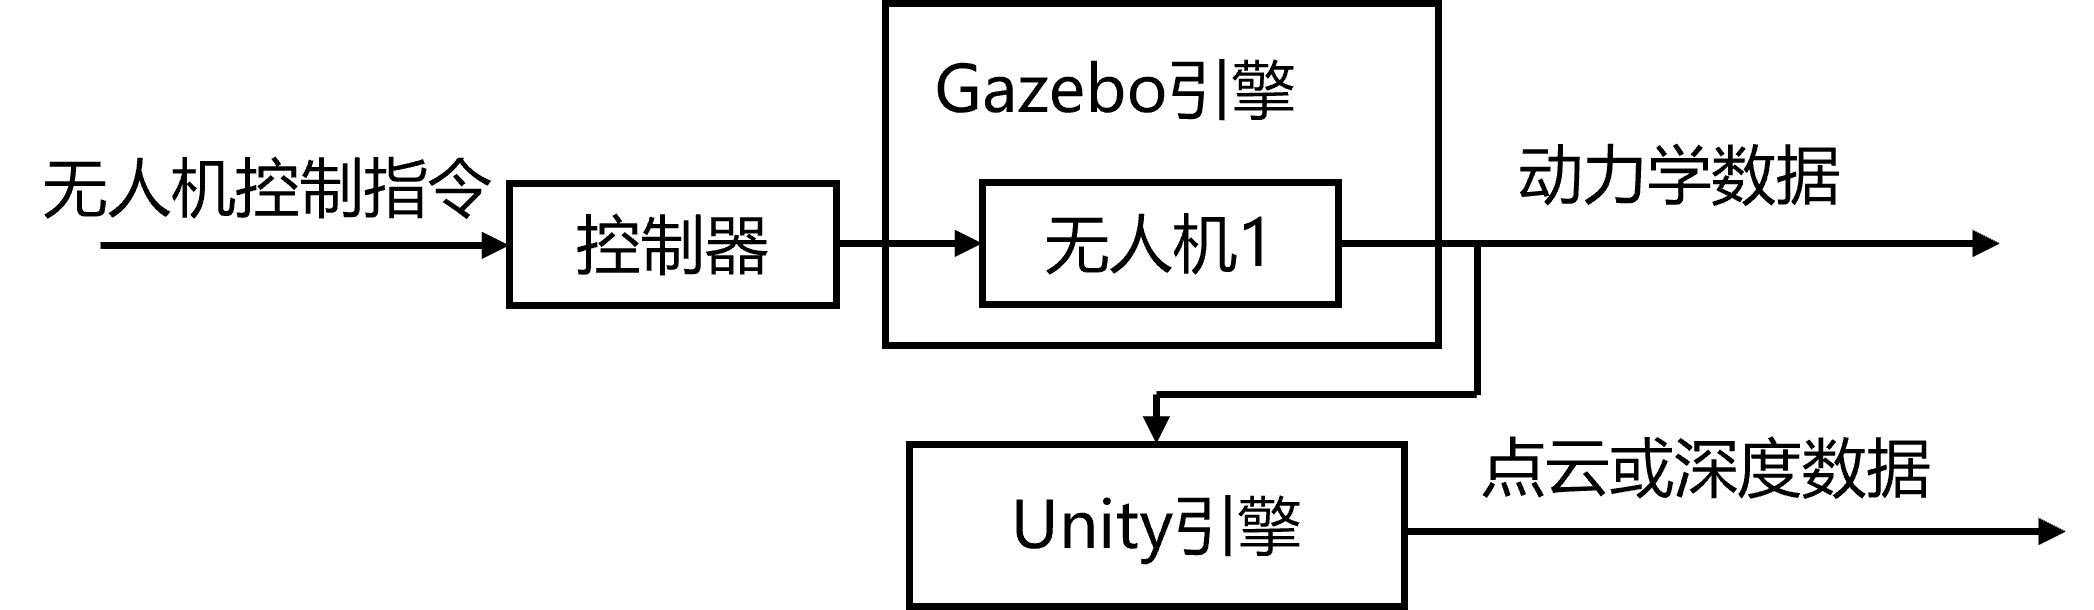
\includegraphics[width = 0.75\textwidth]{simulator_origin.png}
  \caption{FLightmare仿真器结构图}
  \label{fig_simulator_origin}
\end{figure}

\subsection{Gazebo简介}
Gazebo是加州大学提出的机器人仿真平台(平台界面如图\ref{fig_gazebo}所示),可实现对于复杂的室内外环境精确的模拟一个或多个机器人的运动。Gazebo的多体动力学模拟精确,但图形渲染能力羸弱,只能够使用CPU资源仿真简单的传感器模块,随着场景变得复杂,仿真运行速度会急剧降低。
\begin{figure}
  \centering
  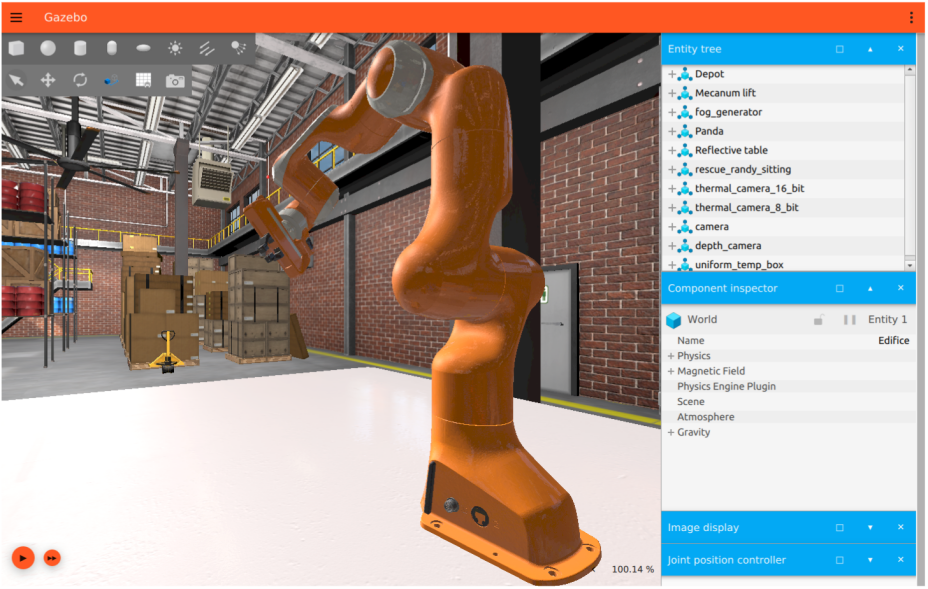
\includegraphics[width = 0.7\textwidth]{gazebo.png}
  \caption{Gazebo物理引擎界面示意图}
  \label{fig_gazebo}
\end{figure}
Gazebo对于ROS生态支持效果较好。因此多出现在使用ROS的仿真平台中。

\subsection{Unity简介}
Unity是一款跨平台的二维和三维游戏引擎\cite{unity},拥有强大的建模和渲染能力。在本仿真器中,Unity主要负责构建场景,并渲染相机、激光雷达等传感器的结果。图\ref{fig_pointcloud}是Unity引擎渲染出树林场景的点云(Pointcloud)数据,图\ref{fig_camera}是同场景对应的图像和深度图像渲染效果。
\begin{figure}
  \centering
  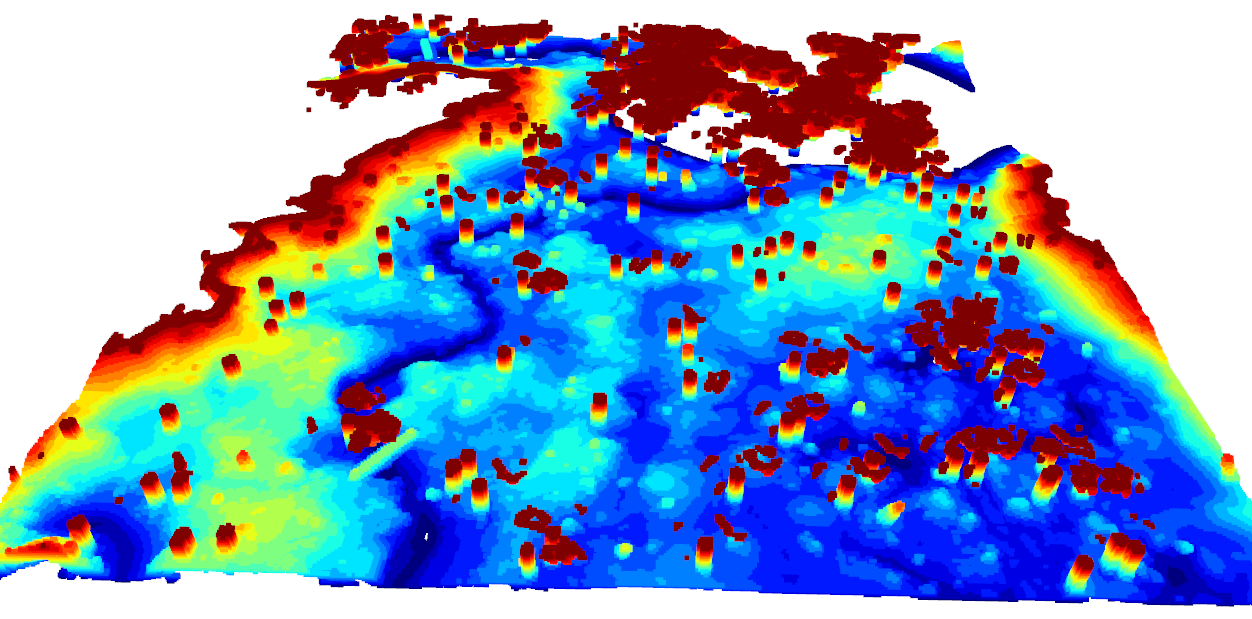
\includegraphics[width = 0.9\textwidth]{pointcloud.png}
  \caption{Unity渲染点云效果示意图}
  \label{fig_pointcloud}
\end{figure}
\begin{figure}
  \centering  
  \subcaptionbox{图像渲染}
    {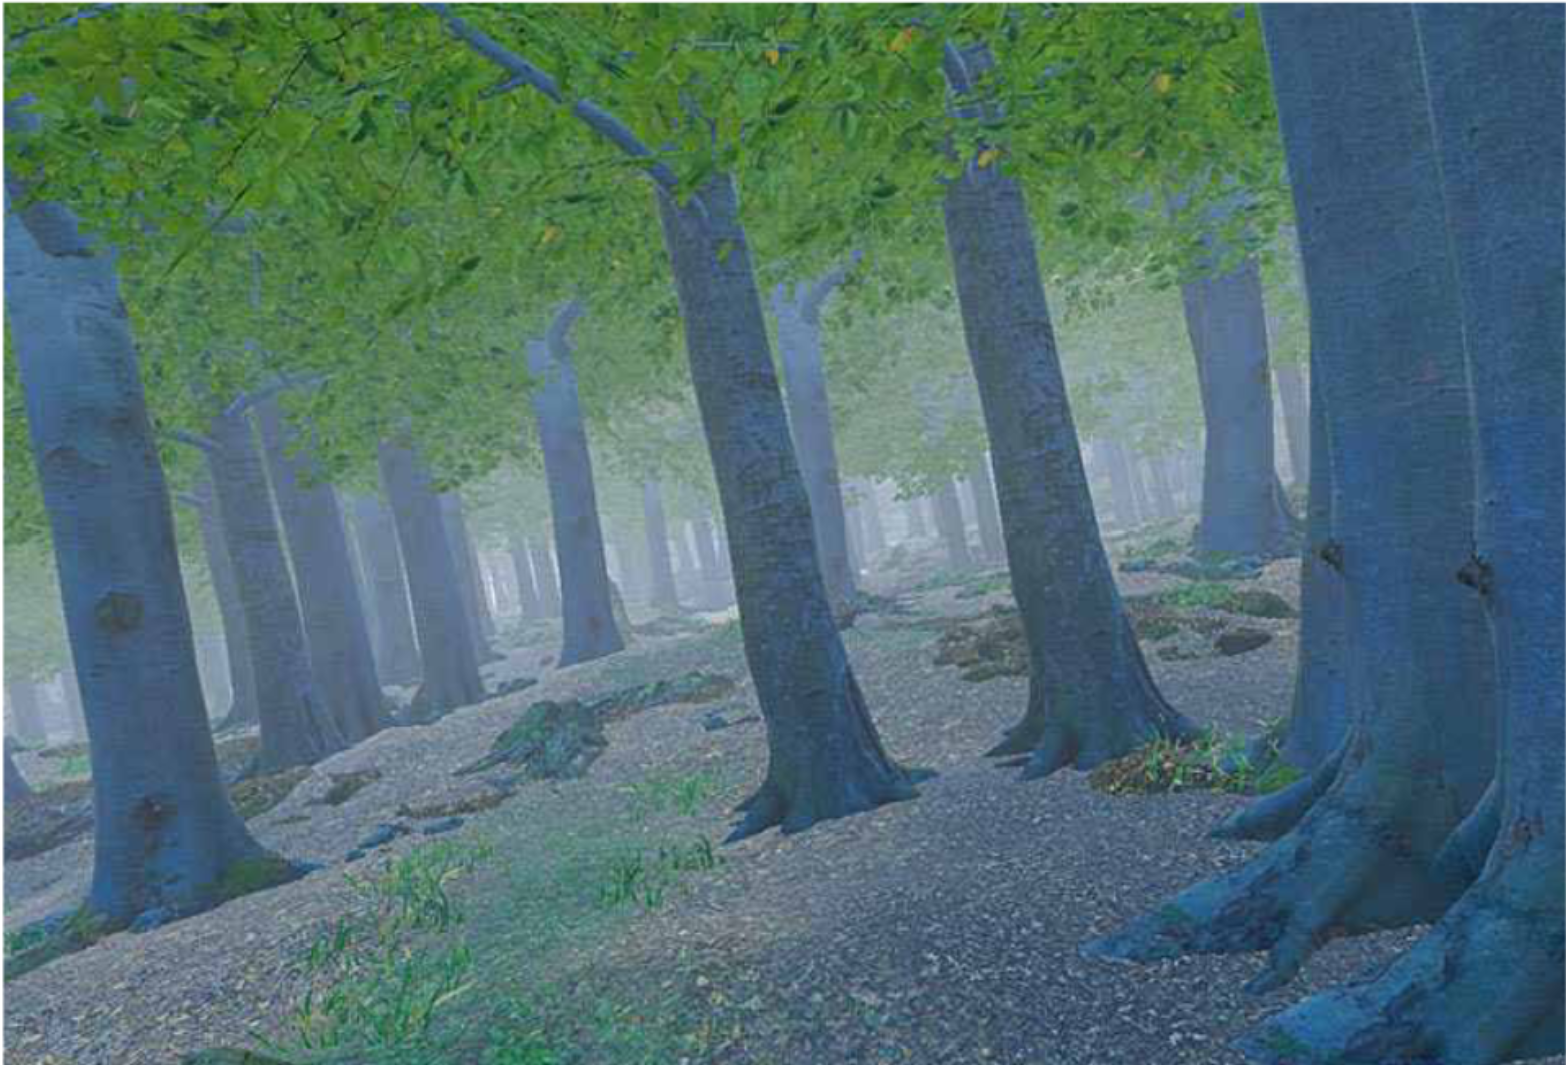
\includegraphics[width=0.45\linewidth]{rgbcamera.png}}
  \subcaptionbox{深度图渲染}
    {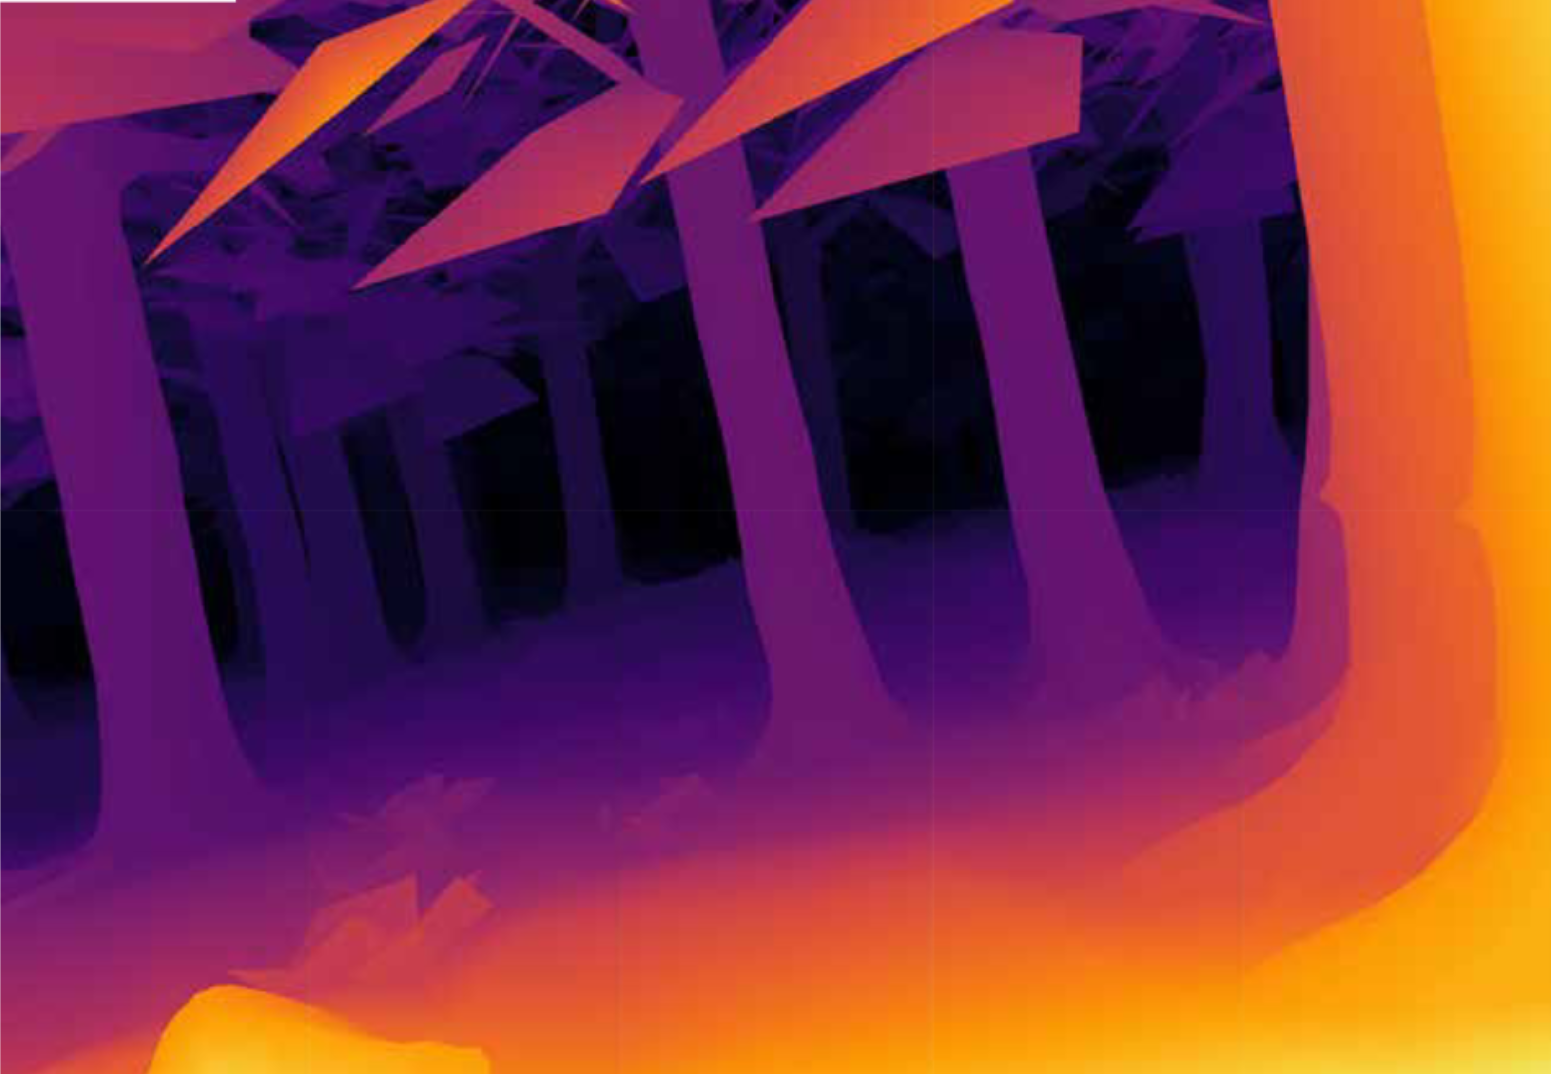
\includegraphics[width=0.45\linewidth]{depcamera.png}}
  \caption{Unity渲染效果示意图}
  \label{fig_camera}
\end{figure}

\section{仿真器加速改进}
\subsection{仿真器加速设计}
本研究利用ROS和Unity的特性通过多线程并行实现了仿真器的加速,具体工作有如下三点:
\begin{enumerate}
  \item 多线程并行Unity,并在Gazebo内并行起飞多架无人机
  \item 使用统一的桥接(Bridge)节点负责Unity和Gazebo的通信
  \item 并行控制器节点为每台飞机提供独立控制
\end{enumerate}

除此之外,受限于单台计算机计算资源,利用ROS的分布式特性还可以在局域网内搭建分布式仿真器结构,进一步加快仿真速度。改造完成的仿真器结构如图\ref{fig_simulator_multi}所示。

在Intel i9 + Nvidia RTX 4090配置的测试平台上实验,改进后的仿真器在每台机器上最多并行2台无人机,通过局域网至多连接3台机器,实现2*3倍并行,训练强化学习算法的速度可提升6倍。
\begin{figure}
  \centering
  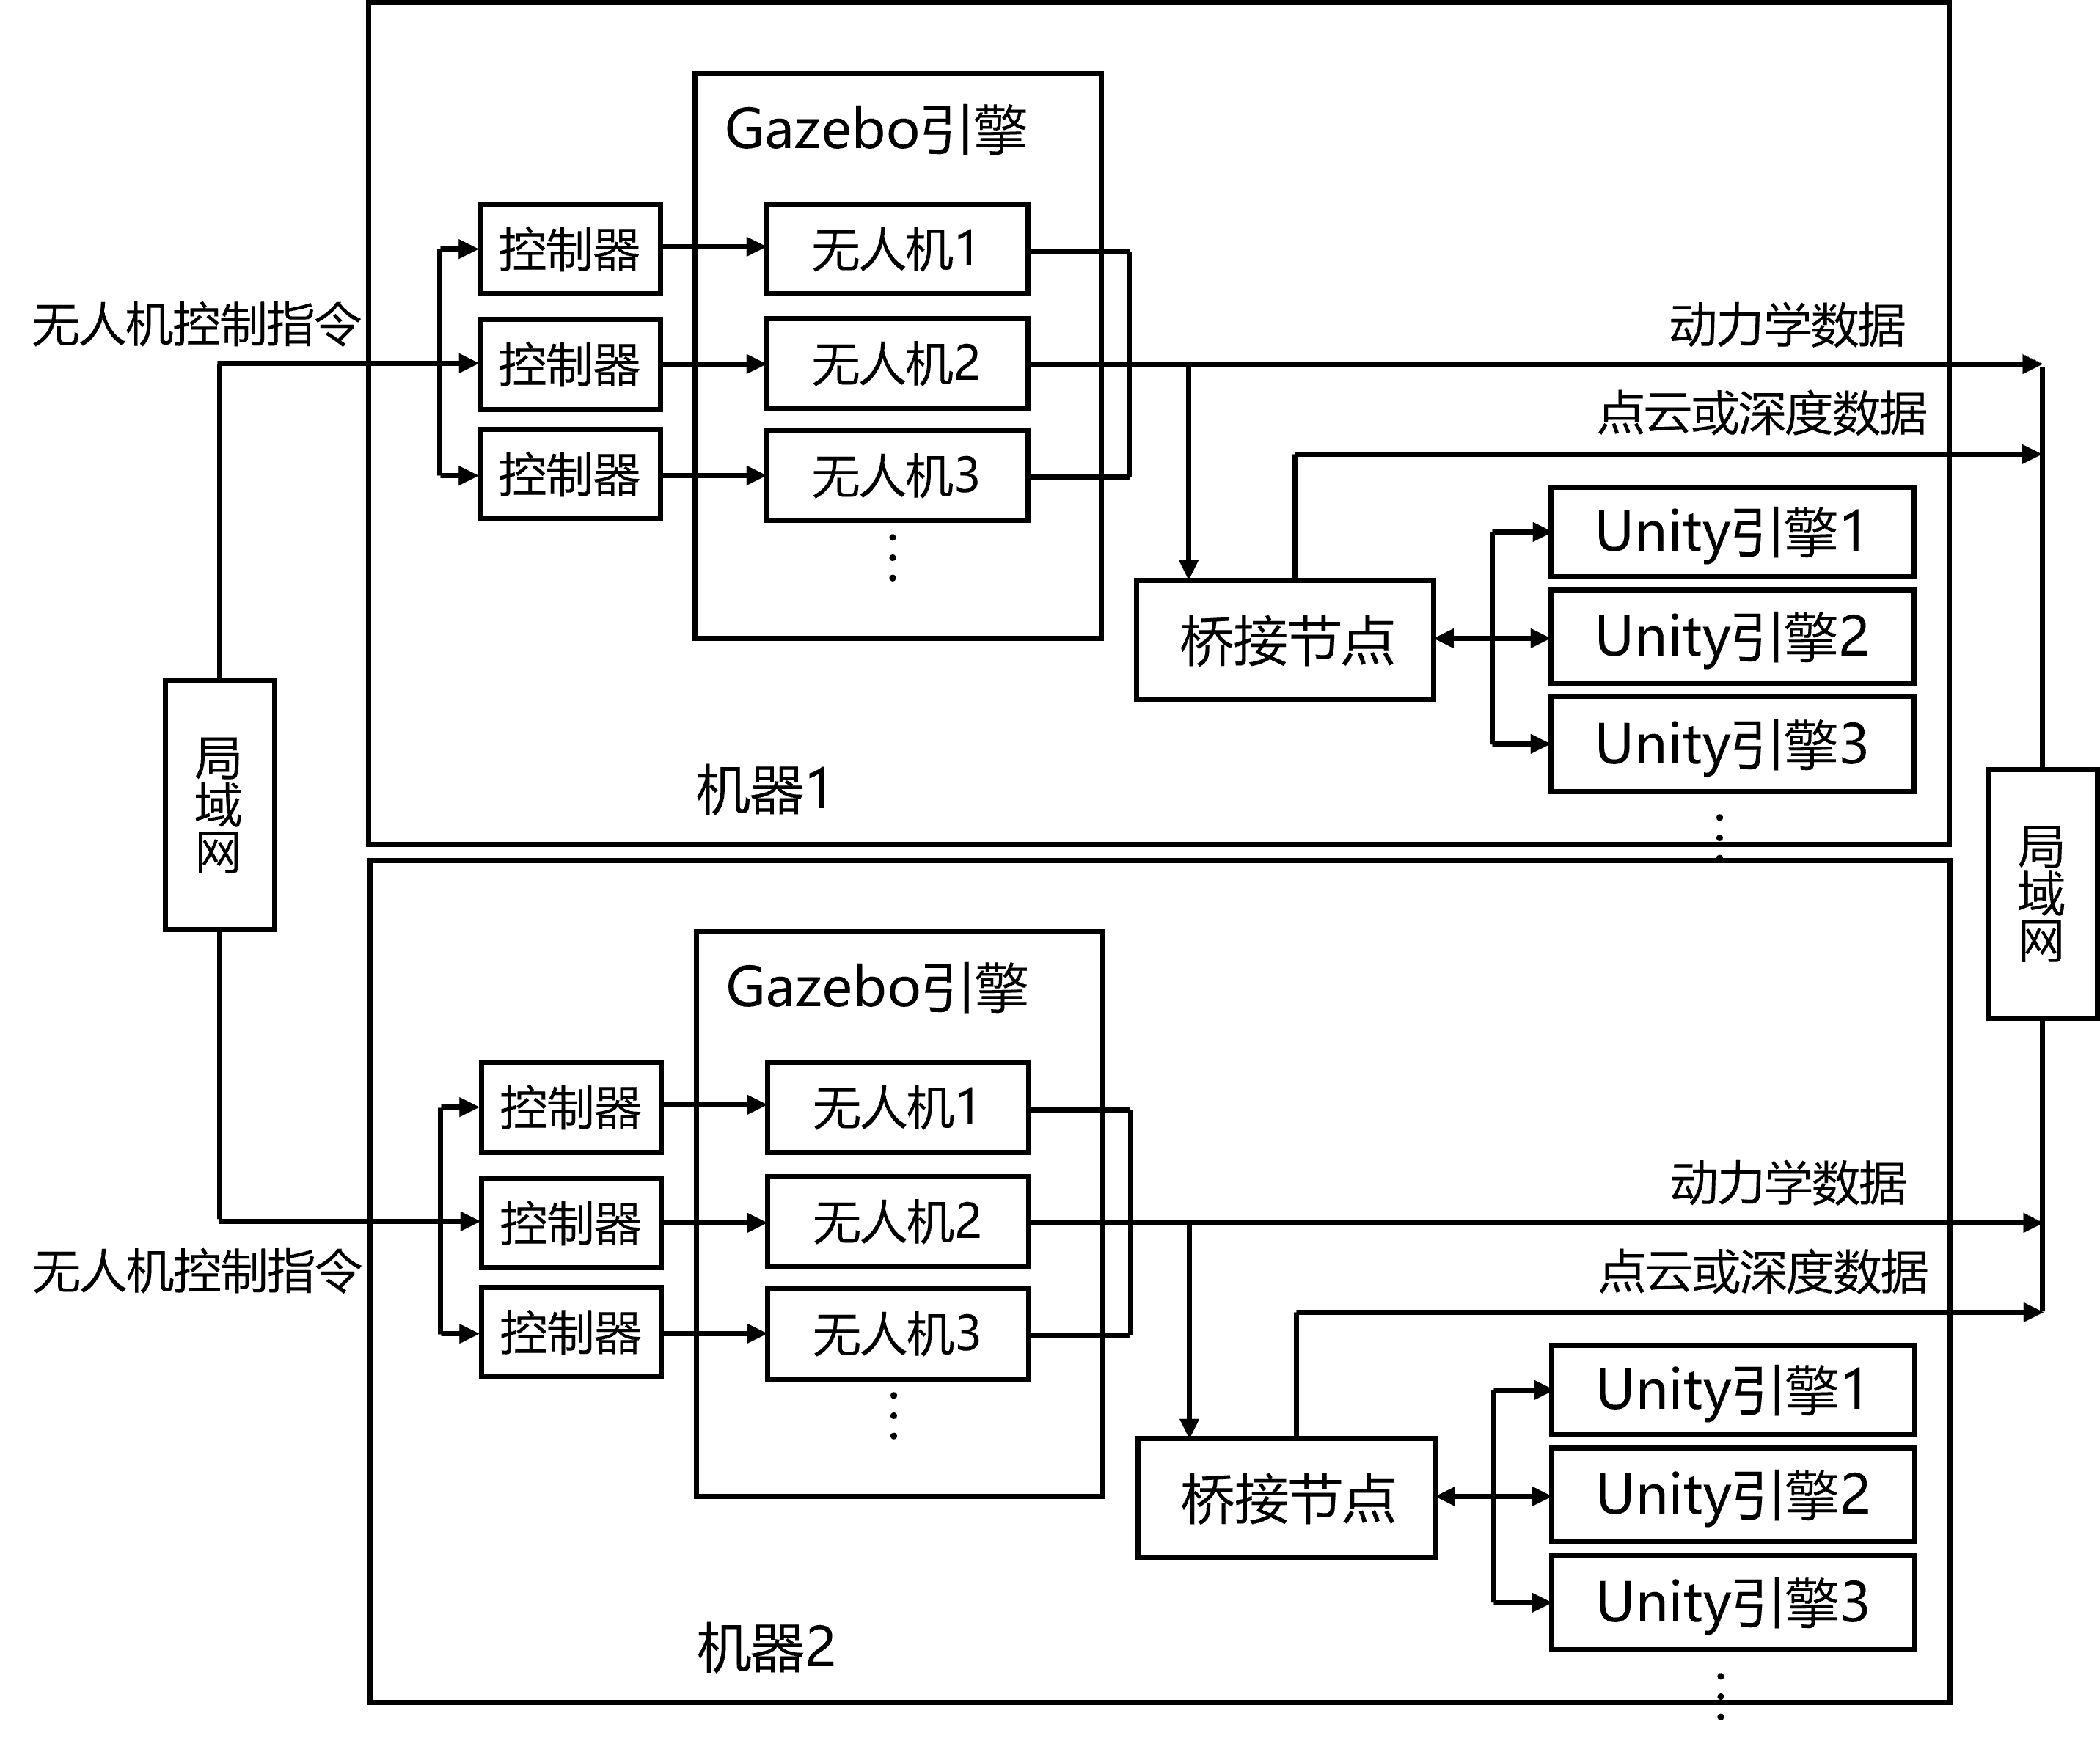
\includegraphics[width = 1\textwidth]{simulator_multi.png}
  \caption{改进后仿真器结构图}
  \label{fig_simulator_multi}
\end{figure}

\section{本章小结}

本章介绍了本研究所使用基础仿真器的基本情况。并介绍了对基础仿真器进行改动的设计。经过并行化设计仿真器的仿真速度得到了大幅提升,为后续算法研究和训练提供了保障。经过测试,改进后仿真器收集算法收敛所需的数据花费的时间约为48$\sim$72小时。


% \section{插图}

% 图片通常在 \env{figure} 环境中使用 \cs{includegraphics} 插入,如图~\ref{fig:example} 的源代码。
% 建议矢量图片使用 PDF 格式,比如数据可视化的绘图;
% 照片应使用 JPG 格式;
% 其他的栅格图应使用无损的 PNG 格式。
% 注意,LaTeX 不支持 TIFF 格式;EPS 格式已经过时。

% \begin{figure}
%   \centering
%   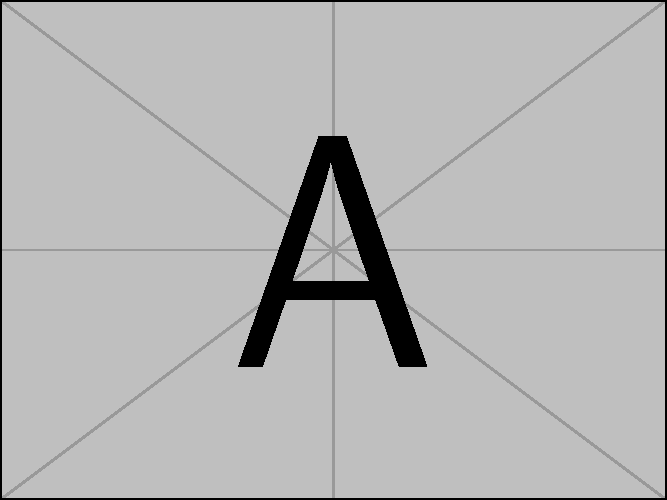
\includegraphics[width=0.5\linewidth]{example-image-a.pdf}
%   \caption*{国外的期刊习惯将图表的标题和说明文字写成一段,需要改写为标题只含图表的名称,其他说明文字以注释方式写在图表下方,或者写在正文中。}
%   \caption{示例图片标题}
%   \label{fig:example}
% \end{figure}

% 若图或表中有附注,采用英文小写字母顺序编号,附注写在图或表的下方。
% 国外的期刊习惯将图表的标题和说明文字写成一段,需要改写为标题只含图表的名称,其他说明文字以注释方式写在图表下方,或者写在正文中。

% 如果一个图由两个或两个以上分图组成时,各分图分别以 (a)、(b)、(c)...... 作为图序,并须有分图题。
% 推荐使用 \pkg{subcaption} 宏包来处理, 比如图~\ref{fig:subfig-a} 和图~\ref{fig:subfig-b}。

% \begin{figure}
%   \centering
%   \subcaptionbox{分图 A\label{fig:subfig-a}}
%     {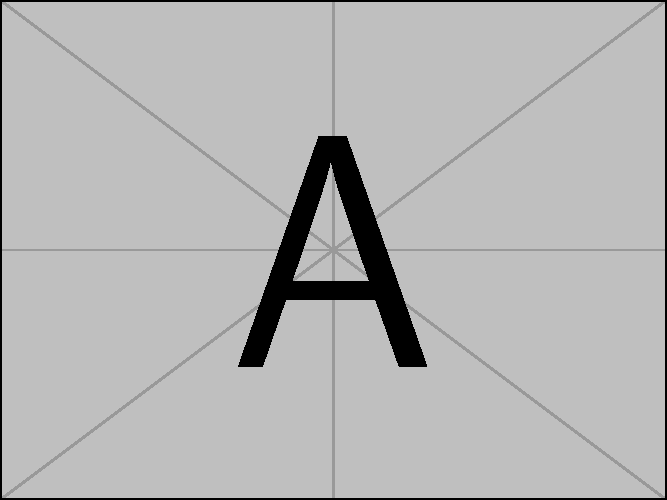
\includegraphics[width=0.35\linewidth]{example-image-a.pdf}}
%   \subcaptionbox{分图 B\label{fig:subfig-b}}
%     {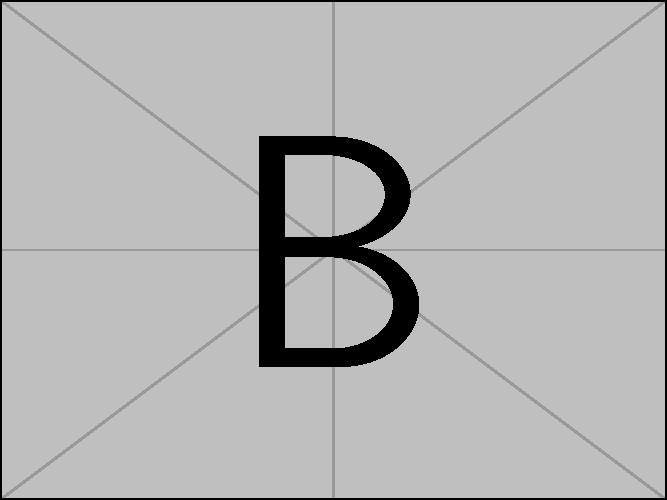
\includegraphics[width=0.35\linewidth]{example-image-b.pdf}}
%   \caption{多个分图的示例}
%   \label{fig:multi-image}
% \end{figure}



% \section{表格}

% 表应具有自明性。为使表格简洁易读,尽可能采用三线表,如表~\ref{tab:three-line}。
% 三条线可以使用 \pkg{booktabs} 宏包提供的命令生成。

% \begin{table}
%   \centering
%   \caption{三线表示例}
%   \begin{tabular}{ll}
%     \toprule
%     文件名          & 描述                         \\
%     \midrule
%     thuthesis.dtx   & 模板的源文件,包括文档和注释 \\
%     thuthesis.cls   & 模板文件                     \\
%     thuthesis-*.bst & BibTeX 参考文献表样式文件    \\
%     \bottomrule
%   \end{tabular}
%   \label{tab:three-line}
% \end{table}

% 表格如果有附注,尤其是需要在表格中进行标注时,可以使用 \pkg{threeparttable} 宏包。
% 研究生要求使用英文小写字母 a、b、c……顺序编号,本科生使用圈码 ①、②、③……编号。

% \begin{table}
%   \centering
%   \begin{threeparttable}[c]
%     \caption{带附注的表格示例}
%     \label{tab:three-part-table}
%     \begin{tabular}{ll}
%       \toprule
%       文件名                 & 描述                         \\
%       \midrule
%       thuthesis.dtx\tnote{a} & 模板的源文件,包括文档和注释 \\
%       thuthesis.cls\tnote{b} & 模板文件                     \\
%       thuthesis-*.bst        & BibTeX 参考文献表样式文件    \\
%       \bottomrule
%     \end{tabular}
%     \begin{tablenotes}
%       \item [a] 可以通过 xelatex 编译生成模板的使用说明文档;
%         使用 xetex 编译 \file{thuthesis.ins} 时则会从 \file{.dtx} 中去除掉文档和注释,得到精简的 \file{.cls} 文件。
%       \item [b] 更新模板时,一定要记得编译生成 \file{.cls} 文件,否则编译论文时载入的依然是旧版的模板。
%     \end{tablenotes}
%   \end{threeparttable}
% \end{table}

% 如某个表需要转页接排,可以使用 \pkg{longtable} 宏包,需要在随后的各页上重复表的编号。
% 编号后跟表题(可省略)和“(续)”,置于表上方。续表均应重复表头。

% \begin{longtable}{cccc}
%     \caption{跨页长表格的表题}
%     \label{tab:longtable} \\
%     \toprule
%     表头 1 & 表头 2 & 表头 3 & 表头 4 \\
%     \midrule
%   \endfirsthead
%     \caption*{续表~\thetable\quad 跨页长表格的表题} \\
%     \toprule
%     表头 1 & 表头 2 & 表头 3 & 表头 4 \\
%     \midrule
%   \endhead
%     \bottomrule
%   \endfoot
%   Row 1  & & & \\
%   Row 2  & & & \\
%   Row 3  & & & \\
%   Row 4  & & & \\
%   Row 5  & & & \\
%   Row 6  & & & \\
%   Row 7  & & & \\
%   Row 8  & & & \\
%   Row 9  & & & \\
%   Row 10 & & & \\
% \end{longtable}



% \section{算法}

% 算法环境可以使用 \pkg{algorithms} 或者 \pkg{algorithm2e} 宏包。

% \renewcommand{\algorithmicrequire}{\textbf{输入:}\unskip}
% \renewcommand{\algorithmicensure}{\textbf{输出:}\unskip}

% \begin{algorithm}
%   \caption{Calculate $y = x^n$}
%   \label{alg1}
%   \small
%   \begin{algorithmic}
%     \REQUIRE $n \geq 0$
%     \ENSURE $y = x^n$

%     \STATE $y \leftarrow 1$
%     \STATE $X \leftarrow x$
%     \STATE $N \leftarrow n$

%     \WHILE{$N \neq 0$}
%       \IF{$N$ is even}
%         \STATE $X \leftarrow X \times X$
%         \STATE $N \leftarrow N / 2$
%       \ELSE[$N$ is odd]
%         \STATE $y \leftarrow y \times X$
%         \STATE $N \leftarrow N - 1$
%       \ENDIF
%     \ENDWHILE
%   \end{algorithmic}
% \end{algorithm}
